\documentclass[a4paper,10pt]{article}
\usepackage{amsmath}
\usepackage{amsfonts}
\usepackage{amssymb}
\usepackage{graphicx}
\usepackage{listings}
\usepackage{algorithm,algorithmic}
\usepackage{float}

\pagestyle{headings}

\newcommand{\IN}{\mathbb{N}}
\newcommand{\MM}{\mathcal{M}}
\newcommand{\QQ}{\mathcal{Q}}
\newcommand{\AAA}{\mathcal{A}}
\title{Rsyslog Design and Internals}
\author{Rainer Gerhards\\
rgerhards@adiscon.com}

\begin{document}

\maketitle

\begin{abstract}
This paper describes rsyslog design and internals. It is created to facilitate a discussion about the implementation of "batched queue processing". As such, it does not describe the full design of rsyslog but rather those elements that are relevant to queues. However, the document may be expanded in the future. This is work in progress and should be considered with care. It is NOT updated during all phases of development.
\end{abstract}

\tableofcontents

\section{Preliminaries}
\subsection{On the Use of English}
\begin{quotation}
\begin{flushright}
I ventured to write this book in English because ... \\
it will be more easily read in poor English, \\
than in good German by 90\% of my intended readers. \\
--- HANS J. STETTER, Analysis of Discretization Methods for \\
Ordinary Differential Equations (1973)
\end{flushright}
\end{quotation}

There is not much I could add to Mr. Stetter's thought, except, maybe, that the number to quote probably tends more to 99\% in this case than to the 90\% Mr. Stetter notes. So please pardon those errors in language use that I have not yet been able to fix or even see. Suggestions for corrections and improvements are always welcome.
\subsection{Notational Conventions}
In general, in rsyslog there exists single objects $o$, which are used to build larger sets $O$, which form a superset $\mathcal{O}$ of all those objects that exist at a given time inside a running instance of rsyslog. As seen above, single objects are always described by lower case letters ($o$), larger sets by upper case letters ($O$) and the ``all-sets'' in caligraphic letters ($\mathcal{O}$). Often, objects $O_i, i \in \IN, i \le |\mathcal{O}|$ partition $\mathcal{O}$, but this is not necessarily the case.

\subsection{Definitions}
\subsubsection{Sudden Fatal Failure}
As sudden fatal failure is one that occurs at some instant and causes Complete loss of processing capabilities. The two major cases are a sudden power loss or a ``kill -9'' of the process. There are more exotic cases, too, like disasters.

One may argue that it is possible to protect against many sudden fatal failure cases. For example, using an uninterruptable power supply (UPS) will prevent a sudden power loss. While this is true in most cases, it does not hold if looked very closely: in the case of the UPS, for example, a failure in the UPS itself may cause a sudden power loss, which can not be mitigated. Well, actually there can be several layers of mitigation, but always one more potential failure scenario remains. So it is not possible to totally solve the issue.

The concept of ``sudden fatal failure'' now covers all these rest risk that result in termiantion of rsyslogd without the ability execute any code before this happens. This is a very important concept in regard to audit-gradeness.

\subsubsection{Audit Grade}
In the context of this document, ``audit grade'' means that a subsystem never loses a message that it has taken responsibility for, not even in cases of sudden fatal failures. The only limit in this restriction is that a subsystem does not guarantee message survival if the subsytem at large is being destroyed (e.g. during a disaster) or some of its components are not of audit-grade. This draws a fine limitation on the audit-grade of a subsystem.

For example, the rsyslog queue subsystem receives messages and acknowledges them to the submitter (e.g. an input), when they have been enqueued in the storage system. If the queue system is configured to provide audit-grade operation\footnote{Audit-grade queue operation is considerably slower than regular operations, as such this mode is not enabled by default. Most installations will never need a completely audit-grade queue}, the queue relies on the storage subsystem to work properly. If, for example, a disk read error occurs, the message may no longer be readable from the disk and as such is lost. The root cause here is that the disk subsystem was not of audit grade, because it otherwise would not have lost the message. So in this case the queue code is of audit grade, but the one of its components, the disk subsytem, was not. So the overall system is not of audit grade.

To simplify talking about the audit-gradness of several subsytems, we assume that all of their subsystems are also of audit grade. In an actual deployment, however, this means the the system designer must carefully select audit-grade subsystems. Overlooking a single non-audit-grade component will make the whole system of not audit grade quality.

Please note that it can be rather tricky to ensure a complete system is of audit grade. A border case is main memory integrity. Even with error-correcting memory, there may situations arise where a memory error occurs (probably due to a very unlikely series of well-hitting cosmic rays) that is unrecoverable. At this point, system integrity is at risk. The only real solution is to immediately shut down the system and restart it (without giving any process a chance to execute). Note, however, that in an extreme view, an operating system routine that does so can also be considered dangerous, as memory in use by this routine might be affected by the malfunction. We could extend this scenario and further complicate it, but that goes beyond the scope of this paper. The example was primarily meant to show how subtle audit-grade reliability is.

In rsyslog, we currently use a slightly \marginpar{duplication\\permitted}relaxed consistency condition for message integrity inside an audit-grade subsystem. While we do not accept message loss, we permit slight message \emph{duplication}, but only in exceptional cases. This is permitted because, with proper message generation, the dulication problem can be easily fixed at the end-to-end layer. For example, the original sender can include a UUID, which can be used to sort out duplicates at the final destination. Insisting on not allowing duplication complicates matters and is often impossible with today's logging protocols. So, for the time being, we aim at this relaxed criteria, which is hard enough to achive. After we have achieved that goal, we may further try to solve the duplicaton problem. Some hooks already exist. But we do not guarantee such an effort will be made any time soon.

\section{Overall Design}
From a high-level prespective, rsyslogd is ``just'' a high-performance message router. It accepts messages from various sources, applies user-configured filters to them, and routes potentially transformed messages to destinations based on these filters.
\section{Objects}
\subsection{Plugins}
Plugins provide code potentially written by a third party to extend rsyslog.

Conceptually, a plugin is a tuple of callable functions $(\phi_1, \phi_2, \ldots)$ which implement an interface. There are three different types of plugins: input, output and library. The plugin type denotes the primary interface implemented by the plugin. Additional interfaces may be implemented\footnote{This is not yet done in plugins, but is possible and assumed to be done at a later point in time}.

In the context of this paper, the output plugin interface is most important. It implements three entry points:

\paragraph{doAction()}
is used to submit messages to the output plugin. The entry point may or may not commit the messages to their ultimate destination.

\paragraph{beginTransaction()}
is used to inform the plugin that a new transaction begins. It must prepare for processing.

\paragraph{endTransaction()}
is indicated that the upper layer \emph{needs} to close the transaction. If there is any uncommited data left, it must be commited or rolled back.

Every instance of an output plugin is guaranteed \emph{not} to be called concurrently by multiple threads. Further, no context switch will happen between calls to $doAction()$ and $endTransaction()$.

\subsection{State Sets}
Several object have associated state based on a specific state set. These state sets are described together with the objects.

As a general rule, individual state is associated with all instances $o$ of a class of objects. This state is called the object's \marginpar{state component} \emph{state component} $s$. If we want to obtain an object's state, we write $S(o)$. Please note that $S(o)$ is only defined for those objects that have a state component.

\subsection{Messages} 
A message $m$ represents a a single syslog message inside the system. It is a tuple of attributes. Some of these attributes directly orginate from the message content, some others are meta-information taken from the context. For example, there is an meta-attribute ``time of reception'' which conveys when the message was received by rsyslog's input subsystem. We do not list attributes here, as there are many and it is not of importance which exactly they are.

The set $\MM$ is composed of all messages that exist at a given time inside rsyslog.

\subsection{Queue}
A queue
$$Q = (C, \Phi, M)$$
is a triplet of a set of configuration parameters $C$, a set of callbacks $\Phi$ and a set of messages $M \subseteq \MM$.

If we need to obtain the set of message from a queue, we write $M(Q)$. The elements of the set of configuration parameters are written as $C_{param}$ where $param$ is an abbreviation of the parameter's meaning. To obtain a specific parameter from a queue, we write $C_{param}(Q)$. The most important elements of $C$ are:

\paragraph{$C_{type}$} which denotes the queue implementation type. Most importantly, this selects from a set of queue drivers (for example disk-only or in-memory driver), which affects the basic operation of the queue instance.

\paragraph{$C_{mMsg}$} which denotes the upper bound on the cardinality of $M$.

\paragraph{$C_{mBatch}$} which denotes the upper bound of the cardinality of message batches created for this queue.

Be $\QQ = \{Q_m, Q_1, Q_2, \ldots, Q_{|\AAA|}\}$ the set of all queues that exist inside rsyslog after the configuration file has been processed, with $|\QQ| = |\AAA| + 1$.

Then
$$M_0 = \MM \setminus \bigcup_{i=1}^{|\QQ|} Q_i(M)$$
\marginpar{at-risk-set}is the set of non-queued messages. The messages have either never been enqueued or have been dequeued but not finally been processed. This set represents the messages that may potentially be lost during an unclean shutdown of rsyslogd. This is why I call this set the ``\emph{at-risk-set}''.


\subsection{Batches}
A batch represents multiple processable messages. It is a unit of processing inside rsyslog's output system. Batches are used to dequeue a number of messages from a queue and then submit them to the lower action layer. Batches are natural \emph{transaction boundaries}, in the sense that multiple output transactions may be done on the messages inside a batch, but each transaction must end at the end of the batch. A batch is always associated to a specific queue $Q$.

A batch
$$B = (b_1, b_2, \ldots, b_n )$$
is a $n$-tuple of \marginpar{processable\\message}processable messages
$$b = (m, s)$$
which are an ordered pair of a message $m$ and an associated processing state $s$. To denote the $n$-th message inside the batch, we write $m(b_n)$, to denote the status component of the $n$-th message, we write $S(b_n)$.

\begin{figure}
\begin{center}
\includegraphics[scale=0.4]{batch_state.jpeg}
\end{center}
\caption{batch message processing states}
\label{fig_batchmsg_states}
\end{figure}

The state set for the processing states is defined as follows:
$$
S_B = \{ rdy, bad, sub, disc \}
$$

With the semantics of the various states being the following:

\begin{center}
\begin{tabular}{|l|l|} \hline
	State		& Semantics \\\hline
	rdy 		& ready for processing\\
	bad		& this message triggered an unrecoverable failure in action\\
			& processing and must not be resubmitted to this action\\
	sub		& message submitted for processsing, result yet unknown \\
	disc		& action sucessfully processed, but must not be submitted \\
			& to any further action in action unit \\\hline
\end{tabular}
\end{center}
The associated state diagram is shown in figure \ref{fig_batchmsg_states} on page \pageref{fig_batchmsg_states}.

Batch sizes vary. The actual cardinality is a function of the cardinality of $M(Q)$ at the time of batch creation and the queue configuration:

$$1 \leq |B| \leq \max(C_{mBatch}(Q), |M(Q)|)$$

\subsection{Action Unit}
An action unit 
$$u = (f, a_1, \ldots, a_n), a_i \in \AAA \text{ for } i \in \IN, i \le n$$
is a tuple consisting of a filter function $f$ and $n \in \IN$ actions. \emph{Does rsyslog still support nonsense action units with $n=0$? - check!}

\subsection{Action}
An action
$$a = (a_C, a_\psi)$$
is an ordered pair of a tuple of configuration attributes $a_C$, and a tuple of processing functions $a_\psi$. Be the set $\AAA$ composed of all actions that exist in rsyslog after the configuration file has been processed.


\section{Processing}
\subsection{Object States}
Various objects keep state. Some of these objects, like messages, batches and actions seem to share state. However, thinking about shared state leads to very complex setup. As such, state is modelled for each object $o$ individually. Instead, the state function $S_O(o)$ can be used to obtain an obtain an individual objects state. That state can be used to modify the state diagrams of the other objects with which relationships exist.

\subsubsection{Actions}
Actions are provided by output plugins. An action enables the engine to write messages to some destination. It is important to note that ``destination'' is a very broad abstraction. A destination may be a file inside a local or remote file system, a database table or a remote syslog server in another network.

Actions are transactional in the following sense: more than one message can be submitted to an action. The action does not necessarily process the submitted messages unless the caller ends the transaction. However, the action itself may also end the transaction and notify the caller. This is \emph{not} considered an error condition and \emph{must} be handled gracefully by the caller. If a transaction aborts, the caller \emph{must} assume that none of the elements submitted since the begin of transaction have been processed. The action will try to backout anything that was already processed at the time the transaction failed. However, not all outputs work on actually transactional destination. As such, an action is permitted not to backout incomplete interim results. As such, after a transaction abort, some message duplication may occur. We call this the \emph{relaxed integrity condition} for actions.

An output transaction is started by calling \emph{beginTransaction()} either explicitely or implicitely by a call to \emph{doAction()} without calling \emph{beginTransaction()} before. Then, one or more calls to \emph{doAction()} follow. When the caller intends to finish the transaction, it calls \emph{endTransaction()}. However, the transaction may also be terminated from the action itself in response to a \emph{doAction()} call.

Mathematically, an action transaction builds a totally ordered set of uncommitted messages $M_u$. The order relation is defined over the sequence in which messages are being provided to \emph{doAction()}. At any time a commit is attempted, the full set $M_u$ is committed and may either succeeed completely or not at all (in the sense of the relaxed integrity condition described above). 

A commit is attempted when 
\begin{enumerate}
\item the caller decides to call \emph{endTransaction()} 
\item or earlier if the action decides it needs to commit now (e.g. because of buffers filling up).
\end{enumerate}

In the seconds case, the action may decide to commit all message but the current one or all (this is depending on action logic). So if the action decideds to commit a transaction before the caller calls \emph{endTransaction()}, a set of commited messages $M_c$ is build and $M_u$ is modified. Be $n$ the $n$-th iterated \emph{doAction()} call and $m_n$ the current message of this call, then the sets are build as follows:

\begin{algorithm}
%\caption{}
\begin{algorithmic}
\IF{action commits $m_n$}
	\STATE $M_c = M_u \cup m_n$
	\STATE $M_u = \emptyset$
\ELSE
	\STATE $M_c = M_u$
	\STATE $M_u = \{ m_n\}$
\ENDIF
\end{algorithmic}
\end{algorithm}

In other words, if anything is committed early, it is always the full set $M_u$, with or without the current message. The caller needs to know which messages are already commited. As \emph{doAction()} finishes one transaction and starts a new one in a single call, we can not use action state the let the caller know this happened. So we use our above finding and just convey back if the transacton is still continuing or the current message or all others before it were committed. The caller must then act accordingly. Please note that when an error happens, the whole transaction must still be considered failed. As such, ``partial commit'' states need not to be mixed with failure states.

Please note that the above method leaves a small potential issue unaddressed: if the action does an early commit of $M_u \setminus m_n$, an error happens when adding $m_n$ to the new $M_u$ (like running out of resources), the action would need to convey both the successful transaction as well as the failure state. This is not possible with the current interface. We could use callbacks to provide such notification, but this complicates the code. So, if that situaton arises, the action must temporarily buffer the error condition and convey it as part of either the next \emph{doAction()} call or during \emph{endTransation()} processing. This can be done, for example, by advancing its internal state accordingly.

The state set for a actions is defined as follows:
$$
S_A = \{ rdy, itx, comm, rtry, susp, died \}
$$

With the semantics of the various states being the following:

\begin{center}
\begin{tabular}{|l|l|} \hline
	State		& Semantics \\\hline
	rdy 		& ready, waiting for transaction begin\\
	itx		& in transaction, accept more data \\
	comm		& transaction finished \\
	rtry		& action failed but may be able to recover \\
	susp		& action currently defunctional until timeout expires \\
	died		& unrecoverable error condition occured, no longer usable \\\hline
\end{tabular}
\end{center}

In the associated state diagram in figure \ref{fig_action_states}, we do not include the \emph{died} state, because it is entered whenever a totally unrecoverable error state may occur. This is a very exceptional incident (which most output plugins do not even support), so we have kept the diagram simple.

\begin{figure}
\begin{center}
\includegraphics[scale=0.5]{action_state.jpeg}
\end{center}
\caption{Action State Diagram}
\label{fig_action_states}
\end{figure}

\emph{Note well} that the state diagram describes the action state. It does \emph{not} describe the transaction state. While action- and transaction state are closely related to each other, they are different entities.

The return code of \emph{doAction()} and \emph{endTransaction()} is used to convey the transaction state. As such, it is a function of the actions's current state after processing the request. The mapping is as shown below:

\begin{center}
\begin{tabular}{|l|l|} \hline
	State		& Return Code (RS\_RET\_\ldots)\\\hline
	rdy 		& OK \\
	itx		& COMMITTED (if there was an auto-commit without $m_n$)\\
			& DEFER\_COMMIT (if there was no auto-commit)\\
	comm		& internal state, not to be exposed to upper layer \\
	rtry		& SUSPENDED \emph{(new code needed)} \\
	susp		& SUSPENDED \\
	died		& DISABLED \\\hline
\end{tabular}
\end{center}

For the rest of this document, let's assume there is a function \emph{getReturnCode()} that implements this mapping.

It is important to think about how retries are handled. There is a user-configured per-action upper number of retries $C_r$ and retry interval $C_i$. In \emph{rsyslog v3}, there is no concept of output transactions. As such, only single messages are processed. When a temporary action failure occurs, the action is re-tried $C_r$ times, where the action processing thread is waiting in a \emph{sleep()} $C_i$ operating system API call\footnote{a suitable API is used, not \emph{sleep()} itself}. If the action succeeds during the retry processing, everything continues as usual. If it does not succeed, two things happen:
\begin{itemize}
\item the message is flagged as ``action permanent failure'' (what may trigger backup processing)
\item the action is actually suspended for $C_i$ seconds
\end{itemize}
If then a new message is sent to the action, and $C_i$ seconds have not yet elapsed, the action is flagged as having failed without being re-tried again\footnote{During the analysis for this paper, it was seen that actually $C_r$ retries are attempted in v3, but each of them will never actually re-try the action. This is a software bug, which does not cause any harm and thus will not be fixed in v3. The new implementation in v4 will obviously not inherit this problem}. This is done in an effort to reduce resource utilization and prevent the system from slowing down e.g. by too-many retries to a remote server that went offline.

With transactional output mode in \emph{rsyslog v4}, the logic above can no longer work. First of all, retrying single actions does not help, because all of the current transaction needs to be resubmitted. As such, the upper layers need to be notified of failure. Then, they need to resubmit the batch. In that design, the lower layer needs to return immediately after detecting the failure. Recovery handling is now to be done when the next transaction is started. However, we must make sure that we do not do excessive retries. So retry processing is only to be carried out if it was not tried less than $C_i$ seconds ago.

The required functionality can be implemeted by a \emph{prepareAction} function that readies the action for processing if there is need to do so. That function is then called in all entry points before anything else is done. Then, actual processing is carried out and the resulting action state be used to generate the return code for the upper-layer caller. Find below a rough pseudocode to do so:

\lstset{language=python}
\begin{lstlisting}
def prepareAction():
   if state == rtry:
      try recovery (adjust state accordingly)
   if state == rdy:
      beginTransaction() [output plugin]
    
def processMessage(message):
   prepareAction()
   if state == itx
      doAction(message) [output plugin]
   return getReturnCode()

def doEndTransaction():
   prepareAction()
   if state == itx
      endTransaction(); [output plugin]
   return getReturnCode()
\end{lstlisting}

\subsection{Output Subsystem Layers}
The rsyslog engine is organized in layers, where each layer is represented by the dominating object:

\begin{figure}
\includegraphics[scale=0.75]{rsyslog_output_layers.jpeg}
\label{rsyslog output layers}
\end{figure}

If looking at the data flow, a queue dequeues batches of messages, which are than run through a generic action system and put into output plugins. Note that on the batch layer, only batches are supported as units of work, whereas the action layer is message-oriented but supports transactions of multiple messages. This is done by indicating when a transaction necessarily needs to end (that point being the end of batch from the batch layer).

The plugins can be written by third parties and are roughly comparable to minidrivers. The generic action system provides all complexity of action processing wheras the output plugin provides a limited set of callbacks that enable the generic framework to talk to the actual destination system. As such, writing outputs is a very simple task. However, rsyslog does not limit the creation of very complex outputs, which may be able to offer superior performance for some destinations.

\subsection{Output Failure}
\subsubsection{Cases}
When an output action is called, it may encounter a failure condition. In general, there are two different cases:
\begin{enumerate}
\item action caused failures
\item message-content caused failures
\end{enumerate}.

Failures rooted in the action are things like broken network connections, file systems run out of space or database servers that are down. Most importantly, the failure is not related to message content. As such, it is appropriate to retry the action with the same message until it finally succeeds (assuming that someone restores the system in question to proper operation). We can not expect that the problem is cleared just by discarding the current message and re-trying with the next one.

In my view, action caused failures are the far majority of all failures. For rsyslog versions 3 and below, all rsyslog-provided plugins consider failures to be action-caused and thus potentially recoverable by simple retry. With the only exception being fatal error conditions that render the whole action unusable.

David Lang pointed out, that there may also exist error conditions that are not caused by the action (or the subsystem it talks to) itself, but rather by message data. He provided the following samples where message content can cause permanent issues with action execution:

\begin{itemize}
\item unicode text causing grief
\item dynafile hits a read-only file
\item basicly data-driven things that trigger bugs in the message delivery 
mechanism in some form.
\end{itemize}

As David Lang said ``In an ideal world these would never happen, but for most output types I can think of some form of corrupt input that could cause that message to fail.''.
So this class of failure conditions actually exists. No matter how often the action retry mechanism is called, it will never succeeds (one may argue that the read-only dynafile is fixable, but we could replace that sample with an invalidly generated filename). The proper cure for these actions is to find the offending one and discard it.

In conclusion, actions need to return different error states for these two different types of failures. Traditionally, RS\_RET\_SUSPENDED is returned when an action specific failure is hit. Most existing plugins also do this if a message-related failure occured, simply because they did not yet know that this situation exists. However, plugins also return different error codes, and at least these can be treated to mean message-permanent failures. To support this, a change to plugins is still required, because many simple return SUSPENDED state if anything went wrong (replacing the real error condition with SUSPENDED). A dedicated PROBABLE\_INVALID\_MSG return state is probably useful so that an output plugin can convey back that it consideres the message to be bad. On the other hand, this implies that the plugin must try to detect those, what means that the developer must think about all potential message-causes problems. That approach can be considered unreliable and as such it may be better not to provide such a dedicted state.

\subsubsection{Handling of Failures}
In spite of the two different failure cases, different handling is needed for them. The action-based failure cases can and must be handled on the action level. As transactions abort when a failure occurs, support from the upper ``batch layer'' is necessary in order to handle resending batches of messages.

For message-caused failure cases, the offending message must be found and then be discarded. A complexity here is that while a failure-causing message is being searched for, an action-based failure might occur. In that case, first the action-based failure condition must be solved, before the search for the problem message can continue.

One approach might be that when the action-layer conveys back an action-caused failure (SUSPENDED), the batch layer knows that it simply needs to restart the full transaction (but not start an ``invalid message search''). If a message-based error condition is conveyed back, the batch system can not restart the full batch. Instead, it needs to enter search mode, where it creates partitions of the original batch, and calls itself recursively (at least in theory) on each of the subsets.

Then, the same handling applies until either a failing message has been found or all messages have been successfully processed. Note that in the recursive step, action-based failures are recovered by full batch resubmits. This solves the above-mentioned complexity in a consistent way.

If a binary-search-like method is used to detect failing records\footnote{This was originally suggested by David Lang.}, recursion may not really be an issue, as the recursion depth is limited to $\log_2 |B|$ where $B$ is the message batch.

A message-caused failure can be rooted in one or more messages. One important question is if it is expected that the failure is caused by a single or multiple messages. Both is possible, so it is a question of probability. If we assume that it is more probable that a single messages causes the problems, it is useful to immediately return back to full batch submission of transactions once a problem-causing message has been identified. But then, if there are multiple problem-causing messages inside the batch, we may need many more iterations.

If, on the other hand, we assume that it is more probable that multiple messages cause problems, it may make sense to keep resubmitting only subsets of the batch. However, then the performance is suboptimal if actually only one message was problematic. A solution might be to pick a compromise, e.g. first assume that a single message is problematic, but assume the opposite as soon as a second message with problems has been found.

A potential algorithm for processing $n \le |B|$ messages from batch $B$ is described below. In the pseudocode, a ``processable'' message is one that neither is already committed nor had a permanent failure with this action. The term ``mpf'' means ``message permanent failure'' for this action (this will later be described in a batch state set).

\begin{small}
\lstset{language=python}
\begin{lstlisting}
def submitBatch(B, n):
   foreach processable message in 
           (first [at most] n messages of batch):
      call processMessage
      if action-caused failure:
         retry full batch
      if action-caused permanent failure:
         mark all n messages as mpf
         return
      if auto-commit:
         mark commited messages in batch as committed
      if message-caused failure:
         if n == 1:
            mark message as mpf
            return
         else:
            call submitBatch(B, n/2)
            call submitBatch(B, n/2)
\end{lstlisting}
\end{small}

After submitBatch() has completed, all messages are either committed or in mpf state.

Note that an action-caused permanent failure occurs if an action-caused failure can not be resolved with the operator-configured number of retries. It will never occur if the user configured infinite retries. While an action is suspended, all calls will result in an action-caused permanent failure. Please keep in mind that these will be resubmitted to any backup actions inside the action unit, so the action's ability to cause permanent failure states is vital for a number of use cases (backup syslog server, to name just one).

Batch processing inside an action unit thus can follow these strucuture:

\begin{algorithm}
\caption{processBatch(B)}
\begin{algorithmic}
\FORALL{action $a$ in action unit}
	\IF{execute action only on messages that failed before}
		\STATE $n = |\text{messages in batch in mpf state}|$
		\STATE change mpf state back to ready
	\ELSE
		\STATE $n = |B \setminus \text{msgs with state discard}|$
		\STATE change all message states $\ne$ discard to ready 
	\ENDIF
	\IF{$n >0$ }
		\STATE call submitBatch(B, n) for action $a$
	\ENDIF
\ENDFOR
\end{algorithmic}
\end{algorithm}

\paragraph{Why is it Important to differentiate the failure cases?}
This text originates from the mailing list and must be merged in. I provide it in the form it is, so it will not be forgotten (plus, it conveys the information).

One may think that it is not necessary to differentiate between action-caused and message-caused failures. However, not doing so introduces subtle issues, because 
then you either 

A) do not need the batch logic at all (because the action is configured for
infinite retries)

Or

B) you loose many messages if the action is not configured for infinite
retries and you have a longer-duration outage e.g. on a database server.
Let's say it is offline for a couple of hours, then you lose almost
everything in that period

To prevent this, you need two different retry methods.

One may argue that it is hard to differentiate between the two failure cases. This is correct. Buit I think it mostly depends on the quality of the output module. 

First of all, ``mostly'' implies that there may be some other cases, where it
really is impossible to differentiate between the two. In that case, I would
treat the issue as an action-caused failure. There are two reasons for this:

1) rsyslog v3 currently does this always and not even a single person
complained about that so far. This is an empiric argument, and it does not
mean it caused problems. But it carries the co-notation that this seems not
to be too bad.

2) If we would treat it as message-caused failure, we would no longer be able
to handle extended outages of destination systems, which I consider a vitally
important feature.

When weighing the two, I know of lots of people who rely on 2), in sharp
contrast to knowig noone having problems with 1). So my conclusion is that it is
less problematic to define an otherwise undefinable failure reason to be
action-caused. Even more so as I assume this problem only exists in the
minority of cases.

Now back to the quality of the output module: thinking about databases, their
API is usually very good at conveying back if there was a SQL error or a
connection abort. So while a SQL error may also be an indication of a
configuration problem, I would strongly tend to treat it is a being
message-caused. This is under the assumption that any reasonable responsive
admin will hopefully test his configuration at least once before turning it
into production. And config SQL errors should manifest immediately, so I
expect these to be fixed before a configuration runs in production. So it is
the duty of the output module to interpret the return code it received from
the API call and decide whether the failure is more likely action-caused or
message-caused. For database outputs, I would assume that it is always easy
to classify failures that must be action-caused, especially in the
dominating cases of failed network connections or failed servers.

For other outputs it may not be as easy. But, for example, all stream network
outputs can detect a broken connection, so this also is a sure fit.

For dynafiles, it really depends on how hard the output module is tries to differentiate
between the two failure cases. But I think you can go great length here, too.
Especially if you do not only look at the create() return code, but, iff a
failure occurs, you do more API calls to find out the cause.

So I think the remaining problem is small enough to cause not too much issues
(and if so, they are unavoidable in any case). In conclusion, the two failure states are not only necessary, but can sufficiently sure enough be detected.

\subsection{Random Topics}
I have begun to gather material from the mailing list in this section, because I feel it may be useful for others as well. Right now, the information is well hidden in the mailing list archives and there may be value in combining it all in one place.

Due to the nature of this material, there is no specific organization between the subchapters and also formatting and language doesn't deny its rooting in the mailing list.

\subsection{Reliability of Message Dequeueing}
A batch is actually dequeued when it is taken off a queue. So if at that point we
have a system power failure (for whatever reason), the messages are lost.
While the rsyslog engine intends to be very reliable, it is not a complete
transactional system. A slight risk remains. For this, you need to understand
what happens when the batch is processed. I assume that we have no sudden,
untrappable process termination. Then, if a batch cannot be processed, it is
returned back to the top of queue. This is not yet implemented, but is how
single messages (which you can think of an abstraction of a batch in the
current code) are handled. If, for example, the engine shuts down, but an
action takes longer than the configured shutdown timeout, the action is
cancelled and the queue engine reclaims the unprocessed messages. They go
into a special area inside the .qi file and are placed on top of the queue
once the engine restarts.

The only case where this not work is sudden process termination. I see two
cases:

a) a fatal software bug
We cannot really address this. Even if the messages were remaining in the
queue until finally processed, a software bug (maybe an invalid pointer) may
affect the queue structures at large, possibly even at the risk of total loss
of all data inside that queue. So this is an inevitable risk.

b) sudden power fail
... which can and should be mitigated at another level

One may argue that there also is

c) admin error
e.g, kill -9 rsyslogd
Here a fully transactional queue will probably help.

However, I do not think that the risk involved justifies a far more complex
fully transactional implementation of the queue object. Some risk always
remains (what in the disaster case, even with a fully transactional queue?).

And it is so complex to let the messages stay in queue because it is complex
to work with such messages and disk queues. It would also cost a lot of
performance, especially when done reliably (need to sync). We would then need
to touch each element at least four times, twice as much as currently. Also,
the hybrid disk/memory queues become very, very complex. There are more
complexities around this, I just wanted to tell the most obvious.

So, all in all, the idea is that messages are dequeued, processed and put
back to the queue (think: ungetc()) when something goes wrong. Reasonable
(but not more) effort is made to prevent message loss while the messages are
in unprocessed state outside of the queue.

\paragraph{More reliable can actually be less reliable}
On the rsyslog mailing list, we had a discussion about how reliable rsyslog should be. It circles about a small potential window of message loss in the case of sudden fatal failure. Rsyslog can be configured to put all messages into a disk queue (instead of main memory), so these messages survive such a powerfail condition. However, messages dequeued and scheduled for processing during the power outage may be lost. 

I now consider a case where we have bursty UDP traffic and rsyslog is configured to use a disk-only queue (which obviously is much slower than an in-memory queue). Looking at processing speeds, the max burst rate is limited by using an ultra-reliable queue. To avoid using UDP messages, a second instance could be run that uses an in-memory queue and forwards received messages to the one in ultra-reliable mode (that is with the disk-only queue). So that second instance queues in memory until the (slower) reliable rsyslogd can now accept the message and put it into the reliable queue. Let's say that you have a burst of $r$ messages and that from these burst only $r/2$ can be enqueued (because the ultra reliable queue is so slow). So you lose $r/2$ messages.

Now consider the case that you run rsyslog with just a reliable queue, one that is kept in memory but not able to cover the power failure scenario. Obviously, all messages in that queue are lost when power fails (or almost all to be precise). However, that system has a much broader bandwidth. So with it, there would never have been r messages inside the queue, because that system has a much higher sustained message rate (and thus the burst causes much less of trouble). Let's say the system is just twice as fast in this setup (I guess it usually would be *much* faster). Than, it would be able to process all r records.

In that scenario, the ultra-reliable system loses $r/2$ messages, whereas the somewhat more "unreliable" system loses none - by virtue of being able to process messages as they arrive. 

Now extend that picture to messages residing inside the OS buffers or even those that are still queued in their sources because a stream transport blocked sending them.

I know that each detail of this picture can be argued at length about.

However, my opinion is that there is no "ultra-reliable" system in life, only various probabilities in losing messages. These probabilities  often depend on each other, what makes calculating them very hard to impossible. Still, the probability of message loss in the system at large is just the product of the probabilities in each of its  components. And reliability is just the inverse of that probability.

This is where *I* conclude that it can make sense to permit a system to lose some messages under certain circumstances, if that influences the overall probability calculation towards the desired end result. In that sense, I tend to think that a fast, memory-queuing rsyslogd instance can be much more reliable compared to one that is configured as being ultra-reliable, where the rest of the system at large is badly influenced by this (the scenario above).

However, I also know that for regulatory requirements, you often seem to need to prove that a system may not lose messages once it has received them, even at the cost of an overall increased probability of message loss.

My view of reliability is much the same as my view of security: there is no such thing as "being totally secure", you can just reduce the probability that something bad happens. The worst thing in security is someone who thinks he is "totally secure" and as such is no longer actively looking at potential issues.

The same I see for reliability. There is no thing like "being totally reliable" and it is a really bad idea to think you could ever be. Knowing this, one may begin to think about how to decrease the overall probability of message loss AND think about what rate is acceptable (and what to do with these cases, e.g. "how can they hurt").

\paragraph{Different Use Cases}
As David Lang pointed out, there exist different use cases for different levels of reliability. Most importantly, there exist use cases that do not demand very high throughput but rather ultra-realiability of the queue system. Here, ultra-reliability is just another word for the queue being of ``audit-grade''. Even if the queue provides audit-grade, the overall system is only then of audit-grade when all other components - most notably the transport protocols spoken by the inputs and outputs - are also of audit-grade. Most importantly, this means that an audit-grade system purely based on the IETF syslog protocol series can not be build.

Used together with truly reliable protocols \emph{and} senders that block processing until a final acknowledgement has been received, an audit-grade system can potentially build based on rsyslog. To do so, an audit-grade queue subsystem is required, which is not present in releases less than 4.1.? (most importantly, v2 and v3 do not provide this capability).

\subsection{Audit-Grade Queue Operations}
\subsubsection{Perquisites}
Audit-grade queue operations certain perquisites:
\begin{itemize}
\item rsyslog engine is of version 4.1.? or greater
\item disk-only queue type
\item checkpoint interval set to 1
\item queue is configured to not permit losing any messages\footnote{The queue has several settings that can be used to fine-tune situations in which it may discard messages intentionally. All of these must be turned off. Most importantly, that means the producer is blocked for an infinite time if the queue is full.}
\item queue consumer must also be of audit-grade
\end{itemize}
Only when these prequisites are met, queue operation can be considered of being audit-grade. Note that when message loss in case of sudden fatal failure and similar incidents is acceptable, neither disk-only queues nore a checkpoint interval of 1 is necessary. Such a configuration can also be build with rsyslog v3, which is up to that level.

Note that in the sections below we describe the implementation in broader terms. Most importantly, we do not restrict ourselves to disk-only queue storage drivers. This is important, because it simplifies design and opens the capability to introduce new, possibly faster-performing, queue storage drivers in the future.

But it is important to keep in mind that a concrete queue is only of audit-grade if it matches all the perquisites given here, most importantly with the right configuration.

\subsubsection{Implementation Alternatives}
Messages, or more precisely objects\footnote{While rsyslog deals with messages, the queue is designed to handle any type of thing that is represented as an rsyslog object. This is considered useful as queues may at some time contain other things than just messages, so we keep it generic.}, are enqueued by the queue producer (either an input module or the main message queue's consumer). The enqueue operation is completed only when the message has been successfully accepted by the queue storage driver. Then and only then the producer is permitted to remove the object from its own storage system. A rough sketch is given in algorithm \ref{alg_q_enq}.

\begin{algorithm}
\caption{enqueueObject($o$)}
\begin{algorithmic}
\label{alg_q_enq}
\STATE lock queue mutex
\WHILE{queue is not ready for enqueue}
	\STATE wait on queue to become ready
\ENDWHILE
\STATE call queue store driver to add $o$
\STATE unlock queue mutex
\end{algorithmic}
\end{algorithm}

The dequeue-operation is more complex. We must ensure that each object stays in the queue until it is finally processed. Hereby, an object is finally processed, when processing of it has been completed. Remember that to enhance performance, objects are dequeued in batches of many. So at any given time, multiple messages may be processed, but not necessarily have finally completed doing so. If another worker thread then tries to obtain a new batch for processing, those ``in-process'' message must not be handed out a second time. Also, if a sudden fatal failure occurs during processing, queue operation must restart at the point of last commit. This means that all ``in-process'' messages need to be changed back to ``no processed'' state and be restarted again. In those cases the (acceptable) slight message duplication can occur.

In our design, we differentiate between ``logical'' and ``physical'' dequeuing of batches. If a batch is generated for processing, it is logically dequeued --- in the sense that no other batch generating request will be able to receive another copy of these messages. If no exceptional situation happens, those messages will be processed and thus can be considered consumed under normal circumstances.

However, actual deletion from the physical queue storage happens only after the batch is fully processed. At this point, all objects have been acknowledged by their destinations, which now have the responsibility for the object's survival. Consequently, we can delete them from the queue store. This process is considered the ``physical'' dequeue of the object.

In order to find some simpler terms, we will call the logical dequeue operation just ``dequeue'' and the physical dequeue operation ``delete''. This is consistent with all previous work on rsyslog and thus probably leads to the least surprise when reading older source code and documentation.

A first idea for a deletion is given in algorithm \ref{alg_pdeq_batch_1} (remember that $O(b)$ contains all objects within the given batch $b$, this is \emph{not} $O$-notation and should probably in the future be replaced by something else).

\begin{algorithm}
\caption{deleteBatch($b$), first approach}
\begin{algorithmic}
\label{alg_pdeq_batch_1}
\STATE lock queue mutex
\FORALL{$o \in O(b)$}
	\STATE find $o$ in queue storage
	\STATE remove $o$ and keep queue structures intact
\ENDFOR
\STATE unlock queue mutex
\end{algorithmic}
\end{algorithm}

This algorithm is simple, but requires searching the queue store for the object to be deleted -- a potentially lengthy operation. However, we can improve the searching process if we know more about the inner structure of batch objects. It seems appropriate to dequeue objects in queue-sequential order. A drawback of doing so is that we must prevent other worker threads from trying to dequeue concurrently. This is not really a drawback. We need to guard dequeue operations by a mutex in any case, because otherwise internal structures can not be kept consistent. Practical experience and testing have shown that many small dequeue operations cause a lot of locking contention and as such badly affect performance. So it actually is a welcome enhancement to aquire the queue lock only once for the whole batch dequeue operation. As dequeing is a comperatively fast operation, the lock is not held for extended periods of time.

A first approach to this functionality is shown in algorithm \ref{alg_ldeq_batch_1}. Note that $C_{mBatch}$ is the configured maximum number of elements inside a batch, $i$ is an index to address the objects inside the batch.

\begin{figure}[h]
\begin{center}
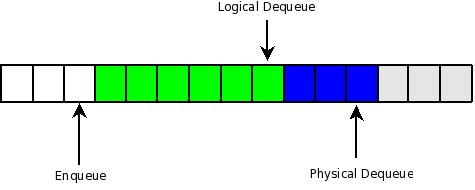
\includegraphics[scale=0.6]{rsyslog_queue_pointers.jpeg}
\end{center}
\caption{\textbf{Queue Store Pointers}: boxes represent queue entries, colored boxes entries with objects. Objects in green are unprocessed, in blue are dequeued but not deleted and those in gray have already been deleted. White indicates not yet used entries. Gray objects may be overwritten at any time. Their entries are actually free, we have used the gray color primarily to indicate there once existed objects. Each queue pointer points to the next entry to process.}
\label{fig_queue_ptr}
\end{figure}

\begin{algorithm}
\caption{dequeueBatch($b$)}
\begin{algorithmic}
\label{alg_ldeq_batch_1}
\STATE lock queue mutex
\STATE $0 \to i$
\WHILE{queue non-empty and $i < C_{mBatch}$}
	\STATE obtain next obj $o$ from queue store 
	\STATE advance logical dequeue position
	\STATE put $o$ into batch
\ENDWHILE
\STATE unlock queue mutex
\end{algorithmic}
\end{algorithm}

A key concept is somewhat hidden in \marginpar{queue pointers} \emph{advance logical dequeue position}. Each queue store is purely sequential, with objects being enqueued at one ``end'' of the store and dequeued at the other. Of course, each queue store has only finite capacity, but we ignore this to explain the overall picture. A queue can be implemented by two pointers: one that points to the tail of the queue, where new messages are enqueued and one that points to the head of it, where new messages are dequeued. The idea is now to duplicate the dequeue pointer and split it into one for (logical) dequeue and one for deletion. Figure \ref{fig_queue_ptr} shows this three-pointer approach. Now, we can simple advance either the dequeue or deletion pointer, depending on operation, and do not need to find the first dequeue position inside the queue store. The dequeue pointer always points at it. This mode can be implemented with all currently existing queue storage drivers (but the sequential disk driver may need to use a second file handle or stream object instead of two pointers).

This makes an efficient implementation of algorithm \ref{alg_ldeq_batch_1} possible: when it logically dequeues, it just needs to advance the dequeue pointer. So the algorithm executes in $O(n)$ time where $n$ specifies the number of elements to dequeue with an upper bound of $C_{mBatch}$.

\begin{figure}[h]
\begin{center}
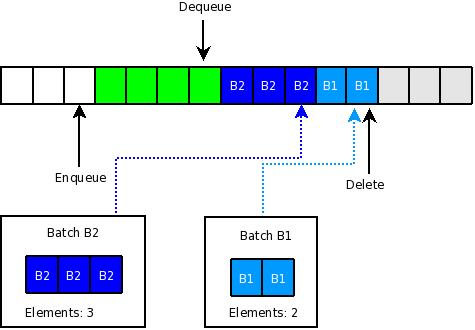
\includegraphics[scale=0.6]{rsyslog_queue_pointers2.jpeg}
\end{center}
\caption{\textbf{Physically Dequeueing Messages}: In this sample, we have two batches. With multiple workers, they may be deleted in any order.}
\label{fig_queue_ptr_deq}
\end{figure}

Furthermore, we can also improve algorithm \ref{alg_pdeq_batch_1}: Consider that each batch is logically dequeued as an atomic operation. That means all batch objects form a sequential subset of the queue. Figure \ref{fig_queue_ptr_deq} shows the situation when two batches have been dequeued.  So the costly ``find'' operation now needs to be carried out only once at the beginning of the batch. As all other objects are sequential, once we have found the batch begin inside the queue, we can simply delete the $|b|$ elements in queue-sequential order after it. So the cost of the find operation can be reduced from $O(|b|)$ to $O(1)$.

We can even reduce the remaining cost of the find operation. If the batch to be deleted is right at the queue's head (as is ``B1'' in the figure), the ``find'' immediately terminates with the first element and incurs no cost at all. The situation is different if the batch is not at the queue head, ``B2'' is an example for that (assuming that ``B1'' has not yet been dequeued). We would now still need to search over the objects that are not part of the batch and can then finally get to the object at the head of the batch in question. For queue storage drivers that support random access to queue elements, storing a simple pointer to the batches' queue head element further improves the situation and enables $O(1)$ access to the queue element. This is indicated by the dotted lines in figure \ref{fig_queue_ptr_deq}. Once the head of the queue has been found, two things can happen (depending on the capabilities of the queue storage driver):

\begin{enumerate}
\item the head element can be flagged as ``this and next $n$ elements are deleted''
\item all elements are actually deleted
\end{enumerate}

Note that a mixed form is also possible (and probably useful for our \emph{singly} linked list storage driver: there, some $n'$ elements be actually deleted and the head element is flagged as ``this and next $n - n'$ elements are deleted''. Note that in the linked-list case, all but the first elements can be deleted with ease\footnote{It can be considered to change from a singly-linked list to a doubly-linked list, if the benefit outweighs the extra effort required.}, so probably just the head would stay inside the queue. Note that removing elements off the queue, where possible, is useful because it frees resources. On a busy system, freeing messages as soon as possible can prevent message loss (in non-audit-grade setup) or system slowdown. So it should be done when possible.

If we have a purely sequential queue storage driver (currently the sequential disk driver), finding and updating the head element is not an option. Even in this case, we can observe that the batch at the actual deletion pointer will eventually be submitted for deletion. So a route to take is to create a list of elements that can be deleted as soon as the physical dequeue pointer reaches any of these elements. We call this the \marginpar{to-delete list}``to-delete list''. To facilitate processing, this list must be ordered in sequence of dequeing. This information may not be available from the storage subsystem itself, but it can easily be generated. To do so, a strictly monotonically increasing counter is kept with each logical dequeue operation and stored as part of the batch\footnote{As this must be done via the usual computer-implemented modular arithmetic, we must be careful that we do not see repetion of values because of overflows. Each day has $60 \cdot 60 \cot 24 = 86,400$ seconds (ignoring the subleties of UTC). Now let's assume that we have a moderately-busy system with 1,000 messages per second. We further assume, to be on the save side, that each message is processed inside its own batch. So we have $86,400,000$ batches per day. If we now use a typical $32$-bit integer for generating the batch IDs, we the unique range will be used up after
$$\frac{2^{32}}{8640000} \approx 497 \text{ days}$$
days of uninterrupted rsyslog operation. While this sounds somewhat save, it goes down to approximately 10 days of messages are submitted at rate of 50,000 messages per second (which is high, but not unheared of). So it is strongly advised to use 64 bits, which we consider to be save, because for our 1,000 messages per second the range would be exhausted only after
$$\frac{2^{64}}{8640000} \approx 2.135 \cdot 10^{11} \text{ days}$$
which equals approximately $584,500,000$ \emph{years}. So even at a rate of one million messages per second, the range would be sufficient for over 500,000 years of continuos operations -- that should be far sufficient.}
An example: let us assume that ``B2'' was submitted for deletion first. Then, the head of ``B2'' is not at the queue's delete pointer. As such, no action can be carried out immediately. So the batch head pointer is stored into a ``to be deleted'' list. Processing continues. Some time later, batch ``B1'' is submitted for deletion. Now, the head pointer is at the head of the delete list, as such all batch elements are dequeued. Then, the ``to be deleted'' list is checked, and ``B2'' is found in it. Now, ``B2'' is at the head of the (new) deletion pointer and can also be removed. So, ultimately, all messages are physically dequeued. This is more formally describe in algorithm \ref{alg_phys_deq_seq_store}. In that pseudocode, we made a simplification by always putting the to be deleted batch in the ``to-delete'' list, which then enables us to use somewhat more generic code to carry out the work.

Note that there is a price to pay for deletions via the ``to-delete'' list: if a sudden fatal failure happens during processing, the set of duplicate messages is increased. For example, if a fatal failure happens after ``B2'' has been fully processed and scheduled for deletion, but \emph{before ``B1'' is also submitted for deletion}, ``B2'' will be reprocessed after recovery. This would not happen if ``B2'' would have been removed from the queue.

\begin{algorithm}
\caption{deleteBatch($b$)}
\begin{algorithmic}
\label{alg_phys_deq_seq_store}
\REQUIRE queue mutex is locked by caller
\STATE enqueue $b.head, |b|$ in ``to-delete'' list $D$
\COMMENT ``to-delete'' list must be in order of logical dequeue
\WHILE{$D.head = Q.deletePtr$}
	\FOR{$|b|$ elements}
		\STATE delete element at queue head
		\STATE move $q.deletePtr$
	\ENDFOR
	\STATE remove head of ``to-delete'' list
\ENDWHILE 
\end{algorithmic}
\end{algorithm}

\paragraph{Warp-Up of Queue Delete Operations}
When evaluating which route to take, the ``to-delete'' list approach looks elegant for all cases. The negative side effect of potentially increased message duplication currently does not even exist: today, the sequential disk queue storage driver permits only a single worker thread and thus there always will be only one thread at a time. Even if we remove that limitation, message duplication could not be avoided, as stated in the algorithm description above. What remains are the other queue storage drivers. However, they operate in-memory, so message duplication will not happen simply because all messages will be lost on sudden fatal failure. The advantage of limited message duplication only exists in the so-far hypothetical case of a random-access, audit-grade disk queue storage driver. Thus, the decision could be postponed unless that happens (if it ever does).

From a code complexity point of view, the ``to-delete'' list approch is definitely advantagous. Not only because of the reduced number of algorithms required. We also do not need to maintain unique batch IDs and all the logic associated with them.

The other aspect to look at is memory consumption. Assuming that we delete the actual objects, just not their containers inside the queue, extra memory consumption is not really that worse. More importantly, currently only the linked-list queue storage driver can benefit at all, because it is the only driver capable of deleting queue entries in mid-queue. All others, including the array memory driver, do not have this capability.

From a performance point of view, the ``to delete'' list approach looks approximately as good as the others, with some mild better performance for some storage drivers for a non-``to delete'' list approach. This can be mitigated, especially if the potentially somewhat-costly maintenance of the ``to-delete'' list is slightly optimized and the algorithm actually checks if the to be deleted batch is right at the queue's delete pointer position. The improved code simplicity, together with current CPU's code caching, may even result in an otherwise not expected speedup.

In conclusion, we will implement the ``to-delete'' list approach on the queue layer (above the queue storage drivers). However, we will leave the window open to permit overwriting it with queue storage driver specific functionality. How to do this will not be specified now, as there is currently no need and we do not even know if there ever will be. However, we retain the discussion on the various modes as well as the relevant algorithmic discussions and data structurs inside this paper so that it is readily available should need arise. We also think this is important so that everybody later knows that the decision was made based on good argument and not by accident (we consider this useful in another design enhancement attempt).

\paragraph{Processing Sequence} Looking at the processing sequence, we notice that always objects are dequeued, then processed and then deleted. Then, the whole process starts again. In particular, this meanss that after the previous batch has been deleted, the next batch will be dequeued. Now consider that we need to have exclusive access to the queue for both of these operations. As such it seems natural to combine this into a single step, further reducing potential locking contention.

Note that a side-effect of this approach is that messages can be deleted only when a new batch is dequeued. With current design, this means that at least one message must reside inside the queue. Otherwise, the last batch will not be deleted. However, this something that can (and must!) be solved on the queue worker layer, in that it deletes a batch when the queue is empty.

This leads us to the implementation of dequeueBatch() and deleteBatch() shown in algorithms \ref{alg_deq_batch_final} and \ref{alg_del_batch_final}. Note that $l$ is a flag variable that indicates if the queue is already locked.

\begin{algorithm}
\caption{dequeueBatch($b$): final version}
\begin{algorithmic}
\label{alg_deq_batch_final}
\STATE lock queue mutex
\STATE call deleteBatch(b, 1)
\STATE $0 \to i$
\WHILE{queue non-empty and $i < C_{mBatch}$}
	\STATE obtain next obj $o$ from queue store 
	\STATE advance dequeue position
	\STATE put $o$ into batch
\ENDWHILE
\STATE commit queue changes to storage system (if needed, e.g. fsync())
\STATE unlock queue mutex
\end{algorithmic}
\end{algorithm}


\begin{algorithm}
\caption{deleteBatch($b, l$): final version}
\begin{algorithmic}
\label{alg_del_batch_final}
\IF{queue not yet locked (test via $l$)}
	\STATE lock queue mutex
\ENDIF
\FORALL{objects $o$ in $b$}
	\STATE destruct $o$
\ENDFOR
\STATE enqueue $b.head, |b|$ in ``to-delete'' list $D$
\COMMENT ``to-delete'' list must be in order of logical dequeue
\WHILE{$D.head = Q.deletePtr$}
	\FOR{$|b|$ elements}
		\STATE delete element at queue head
		\STATE move $q.deletePtr$
	\ENDFOR
	\STATE remove head of ``to-delete'' list
\ENDWHILE 
\STATE commit queue changes to storage system (if needed, e.g. fsync())
\IF{queue not yet locked (test via $l$)}
	\STATE unlock queue mutex
\ENDIF
\end{algorithmic}
\end{algorithm}

\subsubsection{Queue Stores}
Currently, rsyslog supports three different types of queue store drivers:

\begin{itemize}
\item memory array
\item memory linked list
\item disk sequential file
\end{itemize}

They all provide an abstracted sequential queue store as shown in figure \ref{fig_queue_ptr} on page \pageref{fig_queue_ptr}.

Obviously, some differences exist. Most importantly, the disk sequential file driver does \emph{not} support more than one queue worker thread (in order to prevent excessive disk activity and the subtle issues with rewriting parts of sequential files). So if this driver is used, the queue automatically limits itself to a maximum of one worker thread (even if user configuration settings 

Different queue store drivers have different properties:

\begin{tabular}{|l||l|l|l|}\hline
		&	array 	& linked list		& seqential file \\ \hline
pointer type	& integer index	& memory address	& file number and \\
		&		&			& offset within file \\ \hline
physical access	& random	& random		& sequential \\ \hline
remove middle	& no		& yes			& no \\
elements	&		&			& \\ \hline
access to $n$-th& $O(1)$, index:& $O(n)$, follow	& not supported \\
element		& $n \mod C_{mMsg}$	& pointer links	& \\ \hline
speed		& fastest	& fast			& slow \\\hline
mem overhead	& large		& some			& almost none \\\hline
reliability	& reliable	& reliable		& audit-grade\footnote{if configured correctly}\\
\hline
\end{tabular}

\subsubsection{Implementation}
The actual implementation will be based on algorithms \ref{alg_deq_batch_final} and \ref{alg_del_batch_final}. The rsyslog v3 queue storage driver will be extended one additional method, which permits non-destructive dequeueing of elements. As such, the driver now has the $qAdd()$, $qDeq()$, and $qDel()$ entry points (together with the usual construction and destruction entry points). The queue drivers must support the three pointers for enqueue, dequeue and delete. The ``to-delete'' list will be maintained on the upper queue layer (and not the queue driver layer). This functionality will be optimized so that if a batch to delete is right at the queue's delete pointer, it will immediatly be deleted and not be sent to the ``to-delete'' list. This is especially important with the sequential disk driver, as the condition here always is true (and thus the driver can pretend this in the relevant API without even comparing any pointers -- what would otherwise quite complicated in this driver.

The full list of the queue store driver interface is:

\paragraph{qConstruct} Initializes the queue store.

\paragraph{qDestruct} Destructs the queue store, including all messages that may still be present in it.

\paragraph{qAdd} Enqueue a new object into the queue. Note that this entry point must only be called when the queue is non-full.

\paragraph{qDeq} Non-destructive dequeue of the object at queue head. Dequeue pointer is advanced.

\paragraph{qDel} Delete the object at queue head. Delete pointer is advanced.

Disk queue store drivers may support additional internal functions. However, they should not be exposed to the rest of the queue subsystem.

\begin{figure}
\begin{center}
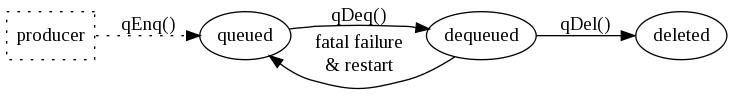
\includegraphics[scale=0.4]{queue_msg_state.jpeg}
\end{center}
\caption{Logical Message States during Queue Processing}
\label{fig_queue_msg_state}
\end{figure}

Figure \ref{fig_queue_msg_state} shows a logical message state diagram during queue processing. There is no actual state variable, but rather the processing flow demands these state. Note that the state transition from ``dequeued'' to ``queued'' only happens after a fatal failure and a successful system recovery. So this is a rather exceptional case.

Another subtle issue is that we now need two different queue size counters: one for seeing when the queue is physically full and one for detecting when there are no more messages to be dequeued.

As a simplification, support for ungetting objects can be removed (as objects never leave the queue), what also means that cancel-processing is probably less complex.

\paragraph{Sequential Disk Queue Store Driver}
The enequeue, deqeueue and delete pointers must be implemented via three stream objects. Most importantly, the dequeue stream must be configured not to delete files when it closes them. A side-effect of this implementation is that data is actually read twice, once to actually obtain it and a second time to delete it. This could only be avoided by an overall redesign on how the disk queue works.

\subsubsection{Checkmarks}
The following things need to be verified in the actual implementation.

\paragraph{Queue Full}
Is it possible to set an infinte timeout on queue full condition during enqueue? If not, we must provide it.

\paragraph{Termination the Queue}
If we cancel a worker, we need to start from the physical dequeue pointer and pull everything that is not scheduled for deletion - NOT from the logical dequeue pointer.

\paragraph{Failed Messages}
If a message fails on a detached action queue, no backup processing is available (because we detect the failure at a point where the message is already considered processed from the main queue's point of view. We need address this and have two options:


I see two approaches at handling this:

a) we enable an action to configure a backup file that shall receive all
message permanent failures. This is simple (not only to implement but to
configure and understand)

b) we push the failed message back to the main queue, but with an indication
that it failed in an action. This is harder to implement and most importantly
harder to understand/configure, but more flexible

\section{Network Stream Subsystem}
The idea of network streams was introduced when we implemented RFC5425 (syslog over TLS) in 2008. The core idea is to encapsulate all stream-oriented network data transfer into a single transport layer and make the upper layers independent of actual transport being used. This is in line with the traditional layer approaches in communication systems.

Under this system, the upper layer provides plugins to send and receive streams of syslog data. Framing is provided by the upper layer. The upper layer itself is integrated in input and output plugins, which then are used to provide application-level syslog message objects to and from the rsyslog core. To these upper layers, the netstream layer provides reliable and sequenced message delivery with much of the same semantics as a usual TCP stream.

\begin{figure}
\begin{center}
\includegraphics[scale=0.4]{tls.jpeg}
\end{center}
\caption{Objects at the Network Stream Layer}
\label{fig_batchmsg_states}
\end{figure}

At the netstream layer, we have a small set of generic classes, which are used for setup of the drivers and driver parameters. This is a very thin layer, mostly a wrapper. Once an actual lower-level netstream driver has been loaded, all parameters are passed through to it.

Please note that both in theory and practice netstream drivers may call back into different netstream drivers. For example, the GnuTLS RFC5425 driver loads and calls back into the plain tcp driver, simply because that driver provides part of the required functionality and there  is no point in re-implementing it for GnuTLS.

The netstream driver layer does not only provide read and write calls but supports i/o multiplexing. To do so, it offers an interface that follows select() semantics. That permits an upper-layer comonent to request being blocked unless some data arrives. Note that due to the subleties in TLS processing, the upper layer may be awoken while there is no upper-layer work to do. This will properly be indicated by the netstream subsystem, is not an error and must be accepted and poperly handled by the upper layer.

Using the nestream layer, we do not need to modify the input and output plugins while at the same time we can add additional transport providers. One weak spot in this design is the current configuration process. With the current system, we need to provide one configuration statement per driver property and we need to hardcode this. So if a new driver would require new properties, we still would need to modify the upper layers. This is unfortunate, but the current config system does not provide for any better way to handle the situation. Once we are able to create a new config system, we will address this by providing the ability to pass a string of parameters onto the driver, which will then have the ability to parse its content. So once we do this, we need to modify the driver interface, but the end result would be a simlification.

So far, only drivers for GnuTLS and plain tcp are provided. However, during the design of the layer we also looked at openssl and Mozilla Network Security Services as well as kept an eye on the needs of Kerberos. In theory, it should not be a major problem to write drivers for these systems (but it most probably still is a lot of work to do).

A final note on Kerberos: in order to keep compatible with previous protocol handling and due to constraints in testing environment and knowledge, we still support Kerberos not via the netstream layer but via special extension into the input and output modules. That, too, is unfortunate, but given the current resources at hand, there is no alternative to handling in that way. We would be very interested in moving over Kerberos to a netstream driver and any volunteer would be very welcome.

\section{Future Development}
This section covers topics that can not currently be developed, but where important thoughts came up in discussions. For obvious reasons, the section has brainstorming character.

\subsection{Audit-Grade High Performance Queue Storage Driver}
An audit grade driver must ensure that no message is lost, but should also be able to handle large workloads. The sequential disk driver does not support the later.

An additional disk driver is envisioned with the properties like the linked list driver, but a reliable on-disk store. In particular, random access to queue elements is desired, which requires an addressing capability.

A potential implementation requires a pre-formatted file. That file is organized in pages of $n$ bytes (e.g. 1K). The page index is used to address a queue item. If an item fits into 1K, it uses one page. If it is larger than 1K, consequtive pages are used to store the element. A page header must be present to indicate how many pages a single element is made up of.

It may be noted that we could even improve performance by keeping part of the data in-memory. For audit-gradeness, it is required that upon enqueue the message is written to disk and only after final processing it needs to be removed. However, it is not forbidden to keep the same message in main memory. That way, the logical dequeue operation could be done one the in-memory representation. Only the physical dequeue would need to write to disk again. As such, we save one disk read out of three writes and one read otherwise required (so one can roughly say that we save one third of disk operations.

Note that due to potential multi-pages messages we can not directly address individual elements, but we can reliably and quikly address elements whom's address we know (learned, for example, during logical dequeue). This is similar to the organization of the in-memory linked list. Actally, such a store \emph{is} a linked list implementation, just that memory is allocated on disk instead of in main memory.

To further improve speed, object representation could be zipped before being written to a page.

File Layout
Page 0: control structures (most importantyle queue pointers) (can make sense to store in a separate file, which could be moved to a dedicated disk subsystem - can potentially greatly reduce disk seek times).
Page 1 to n: actual object storage

Algorithms \ref{alg_AuditGradeStoreEnqueue} and \ref{alg_AuditGradeStoreDelete} show how records are enqueued and deleted. Note that the delete part does not even need to read back the record. If we keep at last some records in-memory, the performance cost of ultra-reliable mode can actually comparatively low. Note that we may not even really need to commit data to the storage system in ``AuditGradeStoreDelete()'', because if a fatal failure occurs at this point, at worst message duplication may happen, what we have considered to be acceptable.

\begin{algorithm}
\caption{AuditGradeStoreEnqueue($o$)}
\begin{algorithmic}
\label{alg_AuditGradeStoreEnqueue}
\REQUIRE queue mutex is locked by caller
\STATE write $o$ to current enqueue location
\STATE update \& write queue structures [page 0]
\STATE sync all files touched 
\STATE store $o$ in an in-memory structure (or a cache)
\end{algorithmic}
\end{algorithm}

\begin{algorithm}
\caption{AuditGradeStoreDelete($o$)}
\begin{algorithmic}
\label{alg_AuditGradeStoreDelete}
\REQUIRE queue mutex is locked by caller
\STATE update queue dequeue pointer \& write queue structures [page 0]
\STATE sync all files touched 
\end{algorithmic}
\end{algorithm}


\end{document}
